The Conceptual models of the system was designed using workflow 
and UML(unified modelling language) diagrams to visualise
behavioural requirments of the automated system. 
The uml diagram was produced using visual paradigm software which provides 
interface to produce digital architecture and system design of software solution. \footnote{\url{https://www.visual-paradigm.com/}}

\subsection{Sequance UML Diagram}
\begin{figure}[!htp]
    \centering
    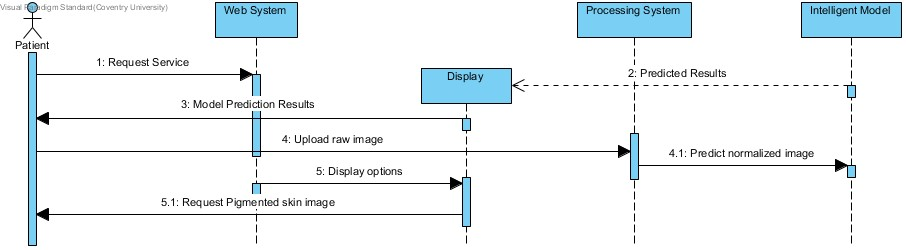
\includegraphics[width=\textwidth]{Images/code.png}
    \caption{Sequance Diagram}
    \label{figure:Sequance}
\end{figure}
The figure \ref{figure:Sequance} represents the sequance uml (unified modelling language) diagram of the 
system. The inital actor in the system is the user or the patient of the 
pigmented skin lesion. The diagram shows the flow of the messages among 
different lifelines in the system. The messages between lifelines outlines the intraction of
the patient with the system in sequantial fashion. Therefore, the diagram helps to capture the 
behavioural requirments of the automated system.
